\documentclass[letterpaper,10pt]{article}

\usepackage{titling}
\usepackage{listings}
\usepackage{url}
\usepackage{setspace}
\usepackage{subfig}
\usepackage{sectsty}
\usepackage{pdfpages}
\usepackage{colortbl}
\usepackage{multirow}
\usepackage{relsize}
\usepackage{amsmath}
\usepackage{fancyvrb}
\usepackage{amsmath,amssymb,amsthm,graphicx,xspace}
\usepackage[titlenotnumbered,noend,noline]{algorithm2e}
\usepackage[compact]{titlesec}
\usepackage[default]{droidserif}
\usepackage[T1]{fontenc}
\usepackage{tikz}
\usetikzlibrary{arrows,automata,shapes,trees,matrix,chains,scopes,positioning,calc}
\tikzstyle{block} = [rectangle, draw, fill=blue!20, 
    text width=2.5em, text centered, rounded corners, minimum height=2em]
\tikzstyle{bw} = [rectangle, draw, fill=blue!20, 
    text width=4em, text centered, rounded corners, minimum height=2em]

\definecolor{namerow}{cmyk}{.40,.40,.40,.40}
\definecolor{namecol}{cmyk}{.40,.40,.40,.40}

\let\LaTeXtitle\title
\renewcommand{\title}[1]{\LaTeXtitle{\textsf{#1}}}


\newcommand{\handout}[5]{
  \noindent
  \begin{center}
  \framebox{
    \vbox{
      \hbox to 5.78in { {\bf ECE155: Engineering Design with Embedded Systems } \hfill #2 }
      \vspace{4mm}
      \hbox to 5.78in { {\Large \hfill #4  \hfill} }
      \vspace{2mm}
      \hbox to 5.78in { {\em #3 \hfill} }
    }
  }
  \end{center}
  \vspace*{4mm}
}

\newcommand{\lecture}[3]{\handout{#1}{#2}{#3}{Lecture #1}}
\newcommand{\tuple}[1]{\ensuremath{\left\langle #1 \right\rangle}\xspace}

\addtolength{\oddsidemargin}{-1.000in}
\addtolength{\evensidemargin}{-0.500in}
\addtolength{\textwidth}{2.0in}
\addtolength{\topmargin}{-1.000in}
\addtolength{\textheight}{1.75in}
\addtolength{\parskip}{\baselineskip}
\setlength{\parindent}{0in}
\renewcommand{\baselinestretch}{1.5}
\newcommand{\term}{Spring 2014}

\singlespace


\begin{document}

\lecture{ 11 --- Multithreading}{\term}{Jeff Zarnett}

\paragraph{Disclaimer} Multithreading is a huge topic and we are not going to be able to cover it in great detail in one lecture. This will come up in much more detail later on in your education, and maybe in your work terms, so this is a small introduction.

\section*{About Multithreading}
The first definition we need to start with is a \textit{process}. A process has three major components: an executable program, the data created/needed by the program, and the execution context of the program (files opened, resources allocated, et cetera). A process has at least one \textit{thread}, and can have many.

The term ``thread'' is a short form of \textit{Thread of Execution}. A thread of execution is a sequence of executable commands that can be scheduled to run on the CPU. Threads also have some state (where in the sequence of executable commands the program is) and stores some local variables. In ECE 150 and most of the other classes you will take at Waterloo, the code you write will have only one thread; that is, your program's code is executed one statement at a time.

A multithreaded program is one that uses more than one thread, at least some of the time. When a program is started, it begins with an initial thread (where the \texttt{main} method is in Java or C\#) and that main thread can create some additional threads if needed. Note that threads can be created and destroyed within a program dynamically: a thread can be created to handle a specific background task, like writing changes to the database, and will terminate when it is done. Or a created thread might be persistent.

See the figure below, which illustrates some possible organizations for processes and threads in different programs:

\begin{center}
	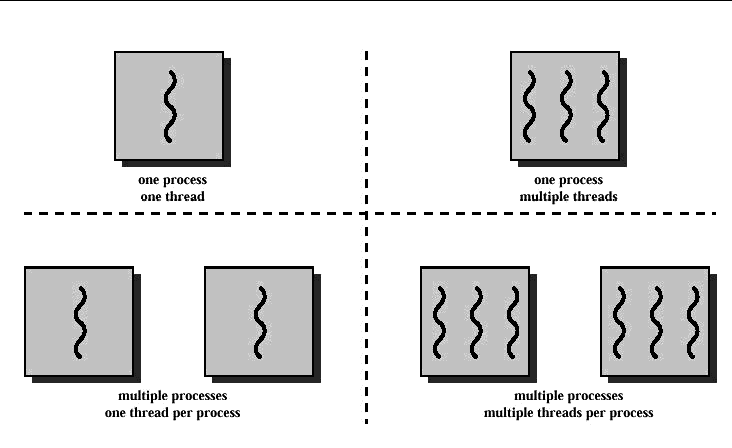
\includegraphics[width=0.525\textwidth]{images/mthread.png} \cite{mthread}
\end{center}

Conceptually, a thread can be in one of three states:
\begin{itemize}
	\item \textbf{Executing} - Currently running.
	\item \textbf{Ready} - Not executing, but it is ready to execute.
	\item \textbf{Blocked} - Cannot execute; waiting for something (like input or resources).

\end{itemize}

The way programs are written now, there are few if any that are not in some way multithreaded. One common way of dividing up the program into threads is to separate the user interface from a time-consuming action. Consider a file-transfer program. If the user interface and upload method share a thread, once a file upload has started, the user will not be able to use the UI anymore (and Windows will put the dreaded ``(Not Responding)'' at the end of its dialog title), even to click the button that cancels the upload. For some reason, users hate that. 

A better design for that file-transfer program would be: when an upload is ready to start, a new thread is created, and that thread will run in the background and upload the file. The UI remains responsive, because the UI thread is not waiting for the upload method to complete. This strategy is even suggested in the official Android guide. You can probably get away without using background tasks in your labs, but it would be more correct if you do intensive computations (e.g., calculating the path the user should walk) in a background task.

\subsection*{Inter-Process Communication}
In most modern operating systems, each process believes that it is running in its own world, where there are no other processes. In older systems where this was not the case, any running process could poke around the memory of another process and see or change what is there. You might encounter this still when dealing with older systems or in certain embedded systems.

Processes can communicate with one another if appropriate set-up is done, but instead of setting up communication between two or more processes, programs commonly use multiple threads. Processes communicating is usually called \textit{IPC} -- Inter-Process Communication. This can be used for message passing, data sharing, or function calls. Some possible ways to set up IPC include files, and shared memory. In the case of Android, IPC can be achieved through \texttt{Intents}, shared memory, or through the \texttt{Binder} class.

Intents are fairly abstract: it is a data container and we can use it to send out a request for another process to do something. You can define it explicitly and say exactly which component should deal with this. More commonly, implicit intents are given to the Android operating system; the operating system will then look for components which can handle this type of Intent \cite{vogella}. If there is more than one program that can handle the Intent, the user gets a popup (example: you click on a link to YouTube and the popup occurs asking if you want to open the link in your browser or in the YouTube app). 

The Binder is quite complex; you may think of it as a client-server model for communication. The details about how the Binder service works are beyond the scope of this course; it is not expected that you will make use of this in your labs.

\subsection*{Processes vs. Threads}

It takes less time to create a new thread than a process, less time to terminate a thread, and switching between threads in the same process is faster than switching between processes. Threads within the same process can share memory and files, and can communicate with each other easily. 

There are some drawbacks, however: there is no protection between threads in the same process. Also, if any thread encounters an error (such as a \texttt{NullPointerException} or Segmentation Fault), the whole process might be terminated by the operating system. If the program has multiple processes for different parts, then the other processes will not be affected; if the program has multiple threads and they all share the same process, then any thread encountering an error might bring the whole thing to a halt.
 

\section*{Execution}
Not that long ago, a typical computer had one processor that could work on one thread at a time. Multiple threads were supported, of course, but the CPU did so by switching between the different tasks. So thread 1 would execute for 20 ms, then thread 2 for 20 ms, then thread 3 for 20 ms, then back to thread 1 for 20 ms. To the user, it seems like threads 1, 2, and 3 are being executed in parallel, because 20 ms is fast enough that the user can't tell the difference.

Now, desktops, laptops, and even cell phones are almost certainly using multi-core processors. A quad-core processor may be executing four different instructions from four different threads at the same time. Time slicing of execution will still occur, if necessary. For example, if there are 10 threads running on a quad-core system, time slicing is necessary to run all those programs.

There's a little bit more to it, however. There are two kinds of ways that different programs and different threads can co-exist in the system: pre-emptive and co-operative multithreading.

\paragraph{Co-operative Multithreading} used to be fairly common, and as hard as it might be to believe, was the way multithreading worked in Mac OS 9. In this system, threads themselves are responsible for yielding the CPU at an appropriate time. The obvious flaw in this, of course, is that there are always some people (programs) that are greedy and never release the CPU. It only takes a small number of misbehaving programs to make the system unusable (or just very unpleasant to use) for others.

The solution, then, is to take the decision out of the hands of the running process and put it in the hands of the operating system. The operating system is much more likely to be fair.

\paragraph{Pre-emptive Multithreading} is the common, accepted standard for multithreading. In this situation, the operating system manages when each thread runs and when it yields the CPU to another thread. Every thread can act as if it is the only thread in the system (and does not need to consider when is a good or bad time to yield the CPU). It just executes.

Although in the vast majority of situations you will encounter pre-emptive multithreading, in embedded systems you may still encounter co-operative multithreading. Usually this is because the embedded system lacks an operating system or the OS is so minimal that it doesn't manage threads. Co-operative multithreading could possibly be more efficient than pre-emptive, if the threads yield the CPU at appropriate times and everyone plays nicely. It is, however, difficult to know when is the best time to yield and there are no guarantees that no-one will try to monopolize the CPU.

\section*{Parallelism \& Speedup}
No doubt it has occurred to you that if there are multiple threads running at the same time, it means a task will get completed faster, right? Well... maybe. It depends a lot on what the task is. There is some overhead involved in splitting a task up and re-combining the results (if necessary), but in most circumstances the overhead is negligible compared to the amount of time working on the task.  

If a task can be fully parallelized, it means the task can be split up in such a way that adding a second executing thread would double the speed of execution. Imagine painting an apartment. It would take one person 12 hours to paint the whole apartment and two people could complete the job in 6 hours. The pattern continues: three people can complete the job in 4 hours, four people in 3 hours, et cetera. This is the ideal, but in the real world there will be a limit to how many additional workers you can add and continue to have this speedup characteristic. At some point, the overhead of adding more threads is no longer negligible. In theory, you could hire 720 painters and finish the job in 1 minute, but at some point you cannot physically fit any more painters into the room.

If a task can be partially parallelized, it means the task can be divided, but doubling the workers doesn't result in completing the job in half the time. Two chefs working together in a kitchen might take 75\% of the time it would take one chef to cook a meal. Adding the extra worker to the kitchen improved the speed at which food was prepared, but it's not doubled. The chefs can work independently some of the time, but at other times one has to wait for the other; the sauce cannot be put on the chicken until the chicken comes out of the oven.

If a task cannot be parallelized at all, then no amount of extra workers will speed it up. Some tasks can only be done sequentially. As the folk saying goes, ``Nine women can't have a baby in one month.''

\subsection*{Bugs}

It can be much harder to convert existing single threaded code into multithreaded code than it is to write multithreaded code in the first place. So if a program will run in multiple threads, it should be designed that way from the beginning, wherever possible.

Multithreaded software is prone to some new types of bugs that single threaded is not. The most likely problem when working with multiple threads is two or more threads trying to update the same piece of data at the same time.

Let's imagine we have an instance of an object \texttt{Location} that has two co-ordinates, \texttt{x} and \texttt{y}. Thread 1 is executing on the left and Thread 2 on the right.

\begin{verbatim}
location.setX(5);                       location.setX(10);
location.setY(7);                       location.setY(0);
\end{verbatim}

Even if each of the set methods is atomic, we cannot guarantee the order in which these operations execute. So we might set \texttt{x} to 5, then \texttt{x} to 10, followed by \texttt{y} set to 0 and then \texttt{y} set to 7. Now our data is inconsistent! There was never a location of $(10, 7)$ in our data set - it should be either $(5, 7)$ or $(10, 0)$, but not half of one and half of another.

We'll get to that subject, and the solutions to the problem, later on in the course when we discuss debugging. 

\bibliographystyle{alpha}
\bibliography{155}


\end{document}
